Este capítulo aborda los términos y definiciones a tener en cuenta y sirve como introducción a Active Directory. En primer lugar, se define la forma en la que los Sistemas Windows gestioana la autenticación y la auterización. Posteriormente, se definen los protocolos de seguridad para la verificación de la autenticación NT Lan Manager y Kerberos. Finalmente, se presenta Active Directory y la terminología necesaria relativa a este.\\

\section{Autenticación y Autorización}

Uno de los principales requisitos a la hora de entender como funcionan la mayoría de los ataques contra Sistemas Windows pasa por la gstión de la autenticación y autorización de los usuarios que inician sesión en el ordenador ya sea a nivel local o en red.\\

Por un lado, la \textbf{autenticación} consiste en la verificación de la identidad de un usuario, dicho con otras palabras, que el sistema de autenticación se asegure de que un usuario es quién dice ser. Por ejemplo, conociendo la contraseña del usuario que dice ser.\\

Por otro lado, la \textbf{autorización} consiste en establacer y delimitar los recursos a los que puede acceder, o no puede acceder ya que los tiene restringidos un usuario (o grupos de usuarios).\\


\subsection{Inicio de sesión interactivo (Interactive Logon)}

El proceso de autenticación a través de inicio de sesión interactivo del inglés {\it Interactive Logon}, a diferencia del inicio de sesión en red o {\it Network Logon}, es llevado a cabo por el proceso {\it WinLogon} que se encarga de recoger las credenciales introducidas por el usuario y su posterior validación. Un usuario que inicia sesión en un equipo ya sea localmente o un inicio de sesión en red introduce el usuario y la contraseña (denominado credenciales de usuario) y sirve para verificar la identidad del usuario. Por otro lado, cuando se inicia sesión a través de una Smart Card {\it (Smart Card Logon)} las credenciales están almacenadas en el chip de la tarjeta y estas son leídas por un dispositivo externo y el usuario introduce el {\it Personal Identification Number (PIN)}~\cite{Capitulo2:Logon}.\\

\subsubsection{Proceso WinLogon}

WinLogon es el proceso encargado de coordinar el inicio de sesión. Además, este proceso también se encarga de gestionar el {\it logout}, lanzar los procesos necesarios para la autenticación de un usuario, cambiar las contraseñas, bloquear y desbloquear un equipo y proporcionar la seguridad necesaria para que ningún otro proceso pueda acceder a información sensible cuando estos procedimientos se están llevando a cabo. 

Como se puede ver en la Figura \ref{WinLogon} el proceso de inicio iterativo consta de varias fases~\cite{Capitulo2:WinInternals}:

\begin{figure}[t!] %[ht!] para here [b] para bottom [t] para top
\begin{center}
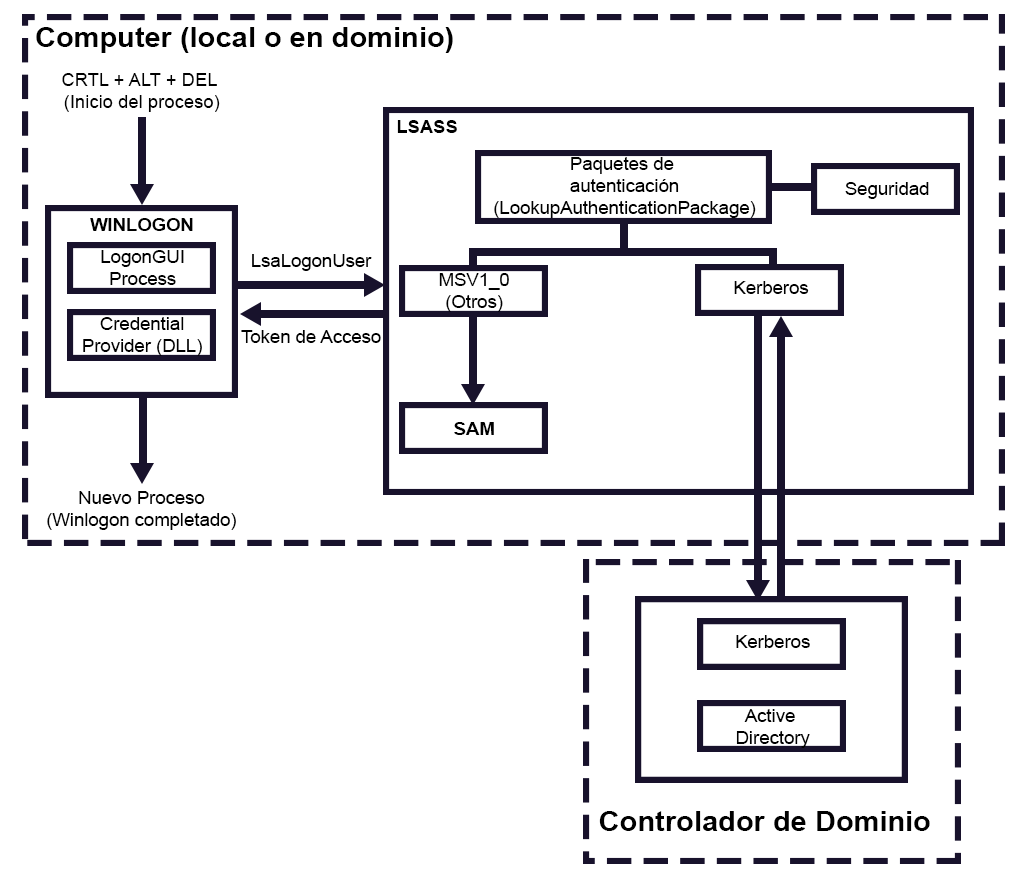
\includegraphics[width=16cm]{WinLogon.png}
\end{center}
\caption{Proceso de inicio de sesión interactivo (WinLogon).}
\label{WinLogon}
\end{figure}

\begin{enumerate}
\item En primer lugar, el proceso de inicio de sesión comienza con una secuencia denominada {\it Secure Attention Sequence (SAS)}, esta secuencia es {\it CTRL + ALT + DEL} por defecto e inicia el proceso WinLogon.
\item Una vez iniciado el proceso WinLogon, este ejecuta el proceso {\it LogonUI} que proporciona la interfaz por defecto para introducir las credenciales y a su vez carga las bibliotecas de enlace dinámico, del inglés {\it Dynamic-Link Library (DLL)} que se encargan de recoger las credenciales y pasarlas al proceso denominado Servicio Subsistema de Autoridad de Seguridad Local del inglés {\it Local Security Authority Subsystem Service} (LSASS). Estas DLLs denominadas {\it Credential Providers} se encuentran en \footnote{\%SystemRoot\%\textbackslash{}System32\textbackslash{}authui.dll} o en \footnote{\%SystemRoot\%\textbackslash{}System32\textbackslash{}SmartcardCredentialProvider.dll} (Si se trata de un inicio de sesión con Smart Cards).
\item Al ejecutarse Winlogon, también se crea un número identificador de seguridad del inglés {\it Security Identifier} (SID), este número se pasa como argumento en la llamada {\it LsaLogonUser} y será incluido en el Token de Acceso {\it (Access Token)} si la autenticación se procesa correctamente. 
\item Una vez introducido usuario y contraseña, WinLogon llama al proceso LSASS a través de la función {\it LsaLookupAuthenticationPackage}. Esta función tiene como objetivo obtener los paquetes de autenticación disponibles en el sistema a través de la clave de registro \footnote{HKEY\_LOCAL\_MACHINE\textbackslash{}SYSTEM\textbackslash{}CurrentControlSet\textbackslash{}Control\textbackslash{}Lsa} como se puede observar en la Figura \ref{Registro-Auth}.

\begin{figure}[t!] %[ht!] para here [b] para bottom [t] para top
\begin{center}
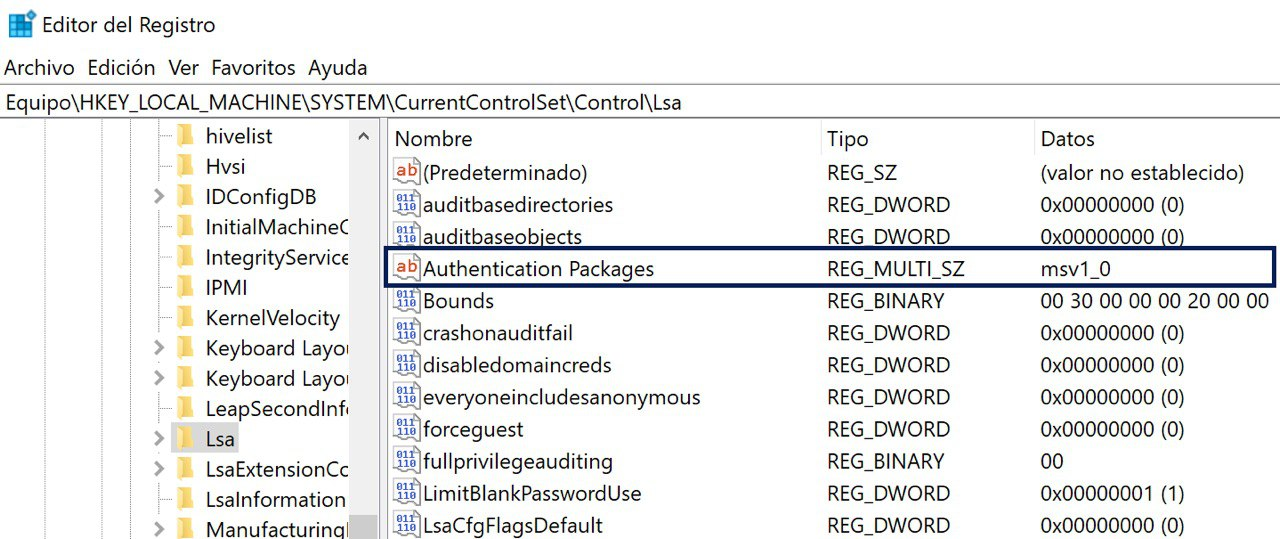
\includegraphics[width=16cm]{Registro-Auth.jpg}
\end{center}
\caption{Clave de registro sobre los paquetes de autenticación.}
\label{Registro-Auth}
\end{figure}

\item Posteriormente, se envían las credendiales a través de la función {\it LsaLogonUser}. Si algún paquete de autenticación autentica el usuario el proceso continua, en cambio, si ningún paquete indica que se ha iniciado sesión correctamente el proceso acaba.

\item Una vez autenticado, el proceso LSASS comprobará en la base de datos de políticas locales si el usaurio autenticado tiene los permisos suficientes para realizar la acción que está solicitando. Si el inicio de sesión no coincide el proceso de autenticación acaba y LSASS elimina cualquier estructura de datos creada y lo notifica a WinLogon. Si el acceso está permitido, LSASS agrega los IDs de seguridad correspondientes, busca en la base de datos los permisos asociados a los usuarios del mismo grupo del SID del usuario y los añade al token de acceso ({\it Access Token}) y crea el Token que será enviado a Winlogon con un mensaje de inicio de sesión correcto. 

\end{enumerate}

Una vez definido el proceso de inicio interactivo a grandes rasgos, se va a pasar a detallar los componentes mencionados que forman parte de dicho proceso.

\subsubsection{Paquetes de Autenticación (Authentication Package)}

\section{NT Lan Manager}

\section{Kerberos}

\section{Active Directory}


